\subsection{Definição e exemplos}

% TODO: rework

Lembre-se que uma \emph{curva}%
\footnote
{
    No contexto da teoria das homotopias, também é muito comum chamar curvas de \emph{caminhos}.
}
entre os pontos $p$, $q$ em um espaço $X$ é dada por uma função contínua $\gamma : I \to X$ parametrizada pelos pontos em um intervalo fechado $I = [a, b] \subseteq \R$, onde $\gamma(a) = p$ e $\gamma(b) = q$. (Para fins ilustrativos, considere p.\@ ex.\@ $X = \R^2$.) Neste sentido, $\gamma$ é uma transformação contínua de $p$ até $q$ no espaço $X$, e informalmente, dizemos que o ponto $p$ é ``deformado'' por $\gamma$, que a deformação resulta em $q$, e que $X$ é o espaço onde ocorre essa deformação. De certa maneira, uma homotopia entre duas funções contínuas $f : X \to Y$ e $g : X \to Y$ representa uma transformação contínua de $f$ até $g$ no espaço $C(X, Y)$; ou seja, uma homotopia $\eta$ entre $f$ e $g$ é intuitivamente uma ``deformação'' de $f$ em $g$ ocorrendo em $C(X, Y)$.%
\footnote
{
    Para valer esta intuição, o conjunto $C(X, Y)$ das funções contínuas de $X$ em $Y$ é considerado um espaço topológico sob a \emph{topologia compacto-aberta}. No caso particular em que $X$ é compacto e $Y$ é metrizável, então a topologia compacto-aberta em $C(X, Y)$ é induzida pela métrica do sup:
    \[
    d(f, g) = \sup_{x \in X} d(f(x), g(x))
    \]
}

\begin{figure}[htpb]
\centering
\begin{tikzpicture}
    \draw [thick]
        (-2,-1)
            node [left] {$p$}
        to[out=45,in=135]
        (1,0)
            node [below left] {$\gamma(t)$}
        to[out=-45,in=-90]
        (2,1)
            node [right] {$q$}
        ;

    \draw [fill]
        (-2,-1) circle (1pt)
        (1,0) circle (1pt)
        (2,1) circle (1pt)
        ;
\end{tikzpicture}
\qquad
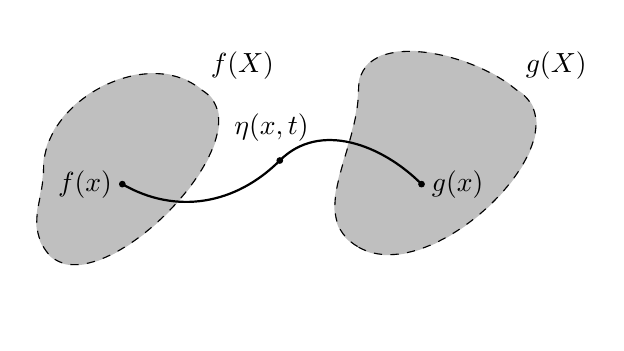
\begin{tikzpicture}

    \draw [fill, lightgray]
        (-2,-1)
        to[out=-60,in=-30]
        (0,1)
        to[out=140,in=90]
        (-2,0)
        to[out=-90,in=120]
        (-2,-1)
        ;

    \draw [dashed]
        (-2,-1)
        to[out=-60,in=-30]
        (0,1)
            node [above right] {$f(X)$}
        to[out=140,in=90]
        (-2,0)
        to[out=-90,in=120]
        (-2,-1)
        ;

    \draw [fill, lightgray]
        (2,-1)
        to[out=-30,in=-30]
        (4,1)
        to[out=140,in=90]
        (2,1)
        to[out=-90,in=150]
        (2,-1)
        ;

    \draw [dashed]
        (2,-1)
        to[out=-30,in=-30]
        (4,1)
            node [above right] {$g(X)$}
        to[out=140,in=90]
        (2,1)
        to[out=-90,in=150]
        (2,-1)
        ;

    \draw [thick]
        %(-0.5,0.5)
        %to[out=45,in=-120]
        %(3.4,0.7)

        (-1,-0.2)
            node [left] {$f(x)$}
        to[out=-30,in=-135]
        (1, 0.1)
            node [above, xshift=-3pt, yshift=3pt] {$\eta(x, t)$}
        to[out=45,in=135]
        (2.8,-0.2)
            node [right] {$g(x)$}
        
        %(-0.8,-0.6)
        %to[out=-45,in=210]
        %(3.2,-0.6)
        ;

    \draw [fill]
        %(-0.5,0.5) circle (1pt)
        %(3.4,0.7) circle (1pt)
        (-1,-0.2) circle (1pt)
        (1, 0.1) circle (1pt)
        (2.8,-0.2) circle (1pt)
        %(-0.8,-0.6) circle (1pt)
        %(3.2,-0.6) circle (1pt)
        ; 
\end{tikzpicture}
\end{figure}

\begin{convention}
    No que segue, e exceto quando explicitamente dito o contrário, $I = [0, 1]$ é o intervalo unitário considerado como um subespaço de $\R$.
    \qedalt
\end{convention}

É fácil ver que toda função $\eta : X \times I \to Y$ do espaço produto $X \times I$ em $Y$ induz uma família $\eta_t : x \mapsto \eta(x, t)$ de funções contínuas de $X$ em $Y$, parametrizada pelos pontos $t \in I$, e pondo $f = \eta_0$ e $g = \eta_1$, temos em adição que $t \mapsto \eta_t$ é uma curva de $f$ até $g$ em $C(X, Y)$; ou seja, $\eta$ induz naturalmente uma ``deformação'' de $f$ em $g$.%
\linebreak\vspace{-1.2em}

Mais que isso: se $\eta$ e $\eta'$ induzem curvas iguais, i.e.\@ $\eta_t = \eta'_t$ para todo $t \in I$, então $\eta = \eta'$. Neste sentido, existe um certo subconjunto de ``deformações'' em $C(X, Y)$ representado unicamente pelas funções continuas $X \times I \to Y$. Obtemos o resultado:

\vspace{0.5em}

\begin{proposition}
    Existe uma injeção natural
    \begin{equation*}
    \begin{gathered}
        \Phi : \{ \text{funções contínuas de $X \times I$ em $Y$} \} \hookrightarrow \{ \text{curvas em $C(X, Y)$} \},
        \\
        \Phi(\eta)(t)(x) = \eta(x, t)
    \end{gathered}
    \end{equation*}
    para todo $(x, t) \in X \times I$ e toda função contínua $\eta : X \times I \to Y$.
    \qedalt
\end{proposition}

Em luz da discussão acima, denominamos a função $\eta$ uma ``homotopia''. Logo:

\begin{definition}[(Homotopias)]
    Sejam $f$ e $g$ funções contínuas de $X$ em $Y$. Uma \emph{homotopia} de $f$ até $g$ é uma função $\eta : X \times I \to Y$ sujeita às seguintes condições:%
    \linebreak\vspace{-1.2em}
%
    \begin{enumerate}
    [
        itemsep=0pt,
        label={(\roman*)}
    ]
        \item
        $\eta$ é contínua.

        \item
        $\eta(x, 0) = f(x)$.
        
        \item
        $\eta(x, 1) = g(x)$.
        \qedalt
    \end{enumerate}
\end{definition}

\begin{convention}
    Por um abuso de linguagem, se $\eta$ é uma homotopia de $f$ até $g$, então às vezes identificamos $\eta$ com a curva $t \mapsto \eta_t$ de $f$ até $g$ em $C(X, Y)$, e dizemos que esta curva é uma homotopia de $f$ até $g$.
    \qedalt
\end{convention}

Considere o seguinte exemplo de homotopia. Sejam $f$ e $g$ funções contínuas de $X$ em um espaço normado $E$. (Para fins ilustrativos, considere p.\@ ex.\@ $X = I$, $E = \R^2$). Fixe $x \in X$ e seja $\gamma_x(t) \in E$ dado para qualquer $t \in \R$ pela equação paramétrica%
\linebreak\vspace{-0.5em}
%
\begin{equation*}
\begin{aligned}
        \gamma_x(t)
    &=  (1 - t) \cdot f(x) + t \cdot g(x)
    \\
    &=  f(x) + t \cdot (g(x) - f(x))
\end{aligned}
\end{equation*}
da reta passando pelo ponto $f(x)$ e na mesma direção do vetor $g(x) - f(x)$. Note que, para $t \in I$, os pontos da forma $\gamma_x(t)$ são exatamente os pontos no segmento de reta entre $f(x)$ e $g(x)$, com $\gamma_x(0) = f(x)$ e $\gamma_x(1) = g(x)$. É evidente que $(x, t) \mapsto \gamma_x(t)$ é contínua e, portanto, uma homotopia de $f$ até $g$. Notavelmente, $\gamma_x : t \mapsto \gamma_x(t)$ é uma família de curvas em $E$, os segmentos de reta entre $f(x)$ e $g(x)$, parametrizada por $x \in X$, e a continuidade dessa homotopia segue da continuidade de $x \mapsto \gamma_x$.%
\linebreak\vspace{-1.2em}

\begin{figure}[htpb]
\centering
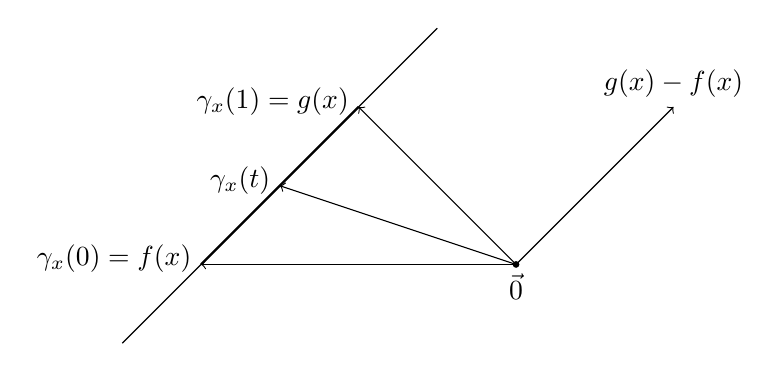
\begin{tikzpicture}
    \draw
        (-5,-2) -- (-1,2)
        ;

    \draw [thick]
        (-4,-1) -- (-2,1)
        ;

    \draw [->]
        (0,-1)
        --
        (2,1)
            node [above] {$g(x) - f(x)$}
        ;
    
    \draw [->]
        (0,-1)
        --
        (-4,-1)
            node [left, yshift=2pt] {$\gamma_x(0) = f(x)$}
        ;

    \draw [->]
        (0,-1)
        --
        (-2,1)
            node [left, yshift=2pt] {$\gamma_x(1) = g(x)$}
        ;

    \draw [->]
        (0,-1)
        --
        (-3,0)
            node [left, yshift=2pt] {$\gamma_x(t)$}
        ;

    \draw [fill]
        (0,-1) circle (1pt)
            node [below] {$\vec 0$};
        ;
    
    
\end{tikzpicture}
\end{figure}

Neste exemplo, a homotopia $(x, t) \mapsto \gamma_x(t)$ é dada por uma família $\{ \gamma_x \}_{ x \in X }$ de curvas em $Y$ indexada pelos pontos em $X$, onde $x \mapsto \gamma_x$ é uma função contínua de $X$ em $C(I, Y)$. Por outro lado, toda homotopia $\eta : X \times I \to Y$ no sentido da Definição 1.2 induz uma ``família contínua'' desta forma, onde $\gamma_x(t) = \eta(x, t)$. Logo:%
\linebreak\vspace{-1.2em}

\vspace{0.5em}

\begin{proposition}
    Existe uma bijeção natural
    \begin{equation*}
    \begin{gathered}
        \Phi : \{ \text{funções contínuas de $X \times I$ em $Y$} \} \iso \{ \text{funções contínuas de $X$ em $C(I, Y)$} \},
        \\
        \Phi(\eta)(x)(t) = \eta(x, t)
    \end{gathered}
    \end{equation*}
    para todo $(x, t) \in X \times I$ e toda função contínua $\eta : X \times I \to Y$.
    \qedalt
\end{proposition}

\begin{convention}
    Dada uma homotopia $\eta$, no que segue denotamos por $\{ \eta_x \}_{x \in X}$ a ``família contínua'' de curvas em $Y$ indexada por $X$ induzida por $\eta$, i.e.\@ onde $\eta_x(t) = \eta(x, t)$, e dizemos que $\eta_x$ é a \emph{componente} de $\eta$ em $x \in X$.
    \qedalt
\end{convention}

\begin{remark}
    Pelas discussões acima, podemos enxergar homotopias como funçôes contínuas $X \times I \to Y$, curvas em $C(X, Y)$, ou ``família contínua'' de curvas em $Y$ indexada por $X$, a depender de qual representação for mais conveniente.
    \qedalt
\end{remark}

Outro exemplo importante de homotopia concerne as curvas em $S^n$ e $B^{n + 1}$, onde
%
\begin{equation*}
    S^n = \{ x \in \R^{n + 1} : ||x|| = 1\},
    \quad
    B^{n + 1} = \{ x \in \R^{n + 1} : ||x|| \leq 1\}
\end{equation*}
%
são subespaços de $\R^{n + 1}$. Como espaços topológicos, dizemos que $S^n$ é uma \emph{$n$-esfera}, e que $B^{n + 1}$ é uma \emph{$(n + 1)$-bola fechada}. Por exemplo, no caso $n = 1$, consideremos as homotopias da curva $\gamma(\theta) = (\cos(\theta), \sen(\theta))$, do círculo unitário centrado em $(0, 0)$, até a curva constante $\msf{const}_p(\theta) = p$ em $p = (1, 0)$, parametrizadas por $\theta \in [0, 2\pi]$.%
\linebreak\vspace{-1.2em}

\begin{figure}[htpb]
\centering
\captionsetup{singlelinecheck=off,justification=centering}
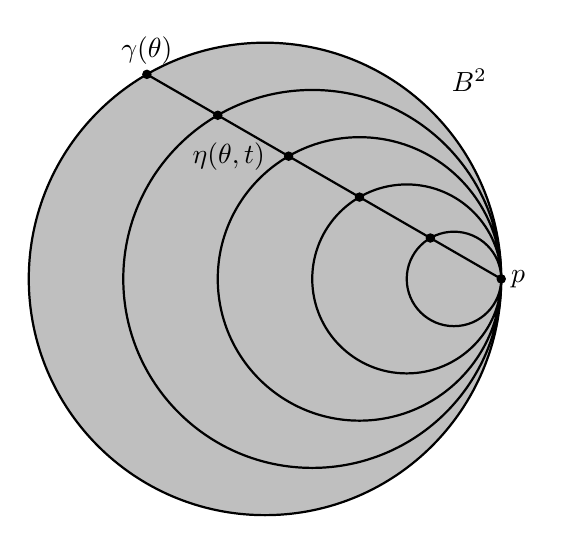
\begin{tikzpicture}
    \draw [fill, lightgray]
        (0,0) circle (3)
        ;
    
    \draw [fill]
        ({3*cos(120)}, {3*sin(120)}) circle (1.5pt)
            node [above] {$\gamma(\theta)$}
        ({2.4*cos(120) + 0.6}, {2.4*sin(120)}) circle (1.5pt)
        ({1.8*cos(120) + 1.2}, {1.8*sin(120)}) circle (1.5pt)
            node [left, xshift=-5pt] {$\eta(\theta, t)$}
        ({1.2*cos(120) + 1.8}, {1.2*sin(120)}) circle (1.5pt)
        ({0.6*cos(120) + 2.4}, {0.6*sin(120)}) circle (1.5pt)
        (3,0) circle (1.5pt)
            node [right] {$p$}
        ;
    \draw [thick]
        (0,0) circle (3)
        ;

    \draw [thick]
        (0.6,0) circle (2.4)
        (1.2,0) circle (1.8)
        (1.8,0) circle (1.2)
        (2.4,0) circle (0.6)
        ({3*cos(120)}, {3*sin(120)}) -- (3,0)
        ;

    \node 
        at (2.25,2.25) [above right] {$B^2$}
        ;
\end{tikzpicture}
~~~
\begin{tikzpicture}
    \draw [fill]
        (3,0) circle (1.5pt)
            node [right] {$p$}
        ;
    \draw [thick]
        (0,0) circle (3)
        ;

    \draw [fill]
        ({3*cos(120)}, {3*sin(120)}) circle (1.5pt)
            node [above] {$\gamma(\theta)$};

    \node 
        at (2.25,2.25) [above right] {$S^1$}
        ;
\end{tikzpicture}
\end{figure}

Para todo $(\theta, t) \in [0, 2\pi] \times I$, o segmento de reta dado pela equação paramétrica
\begin{equation*}
    \eta(\theta, t) = (1 - t) \cdot \gamma(\theta) + t \cdot p
\end{equation*}
está contido em $B^2$ e é uma curva de $\gamma(\theta)$ até $p$, donde segue pelo exemplo anterior que $(\theta, t) \mapsto \eta(\theta, t)$ é uma homotopia de $\gamma$ até $\msf{const}_p$,%
\footnote
{
    Note que, se fixarmos $t$, então a curva $\theta \mapsto \eta(\theta, t)$ descreve um círculo de raio $1 - t$ centrado em $(t, 0)$. Portanto, a homotopia $\eta$ pode ser dada, de maneira equivalente, por uma ``deformação'' em $B^2$, onde o círculo unitário descrito pela curva $\gamma$ é ``contraído'' continuamente até o ponto $p$.
}
e em geral toda curva em $B^2$ é homotópica a uma curva constante por razões similares. Por outro lado, isto não é o caso em $S^1$, e de fato $\gamma$ é um contra-exemplo: não existem homotopias de $\gamma$ até $\msf{const}_p$ em $S^1$. {\it Isto é um fato não-trivial sobre $S^1$}, e nós teremos ferramentas para demonstrá-lo apenas nas seções seguintes, mas podemos vê-lo, intuitivamente, da seguinte forma. Pela Convenção 1.4, uma homotopia de $\gamma$ até $\msf{const}_p$ determina uma família $\eta_\theta$ de curvas em $S^1$ para todo $\theta \in [0, 2\pi]$, com $\eta_\theta(0) = \gamma(\theta)$ e $\eta_\theta(1) = p$. Contudo, contrário à Proposição 1.2, toda tal família contém uma descontinuidade.

Esta descontinuidade ocorre precisamente no interior $B^2 \setminus S^1$ de $S^1$ como um subespaço de $\R^2$. De fato, se considerarmos em particular a homotopia $\eta$ entre $\gamma$ e $\msf{const}_p$ em $B^2$ dada acima, então é fácil ver que (i) para algum $\theta \in [0, 2\pi]$, a curva $t \mapsto \eta(\theta, t)$ intercepta um ponto em $B^2 \setminus S^1$, ou (ii) para algum $t \in I$, a curva $\theta \mapsto \eta(\theta, t)$ intercepta um ponto em $B^2 \setminus S^1$. Em ambos os casos, $\eta$ não é contínua, e em geral, podemos pensar sobre a não-existência de uma homotopia $\eta$ entre $\gamma$ e $\msf{const}_p$ em termos de descontinuidades na família $\{ \eta_x \}$ ou nos seus componentes $\eta_x$.